
\begin{frame}
 \frametitle{Recognition and Tagging : Two step problem}
 \begin{center}
\textcolor{blue}{Michael Jordan is a Professor at Berkeley}
   \end{center}

\end{frame}

\begin{frame}
 \frametitle{Recognition and Tagging : Two step problem}
 \begin{center}
\textcolor{blue}{Michael Jordan is a Professor at Berkeley}
   \end{center}

 \begin{itemize}  
  \item Step 1 : \textbf{Identify} entities

  \medskip
  \textcolor{green}{Michael Jordan\_PERSON} is a professor at \textcolor{green}{Berkeley\_INSTITUTION} \medskip
  
\end{itemize}
\end{frame}

\begin{frame}
 \frametitle{Recognition and tagging : Two step problem}
 \begin{center}
\textcolor{blue}{Michael Jordan is a Professor at Berkeley}
   \end{center}

 \begin{itemize}  
  \item Step 1 : \textbf{Identify} entities
  \medskip
  
  \textcolor{green}{Michael Jordan\_PERSON} is a professor at \textcolor{green}{Berkeley\_INSTITUTION} \medskip
  \item Step 2 : \textbf{Link} entities to knowledge bases : 
  \medskip
  
  \textcolor{red}{Michael Jordan\_ENTITY} (\url{http://en.wikipedia.org/wiki/Michael_I._Jordan})  is a professor at  
  \textcolor{red}{Berkeley\_ENTITY} (\url{http://en.wikipedia.org/wiki/University_of_California,_Berkeley})
\end{itemize}

\end{frame}

\begin{frame}
\frametitle{NER : Problem Statement}
 \begin{center}
\  \begin{definition}[Named entity recognition\footnote {from \ref{thewiki}}]
   Named-entity recognition (NER) (also known as entity identification and entity extraction) is a subtask of information extraction that seeks to locate and classify 
   atomic elements in text into predefined categories such as the names of persons, organizations, locations, expressions of times, quantities, monetary values, percentages, etc.
  \end{definition}

 \end{center}
\end{frame}

\begin{frame}
 \frametitle{NER : Solutions}
 \begin{center}
 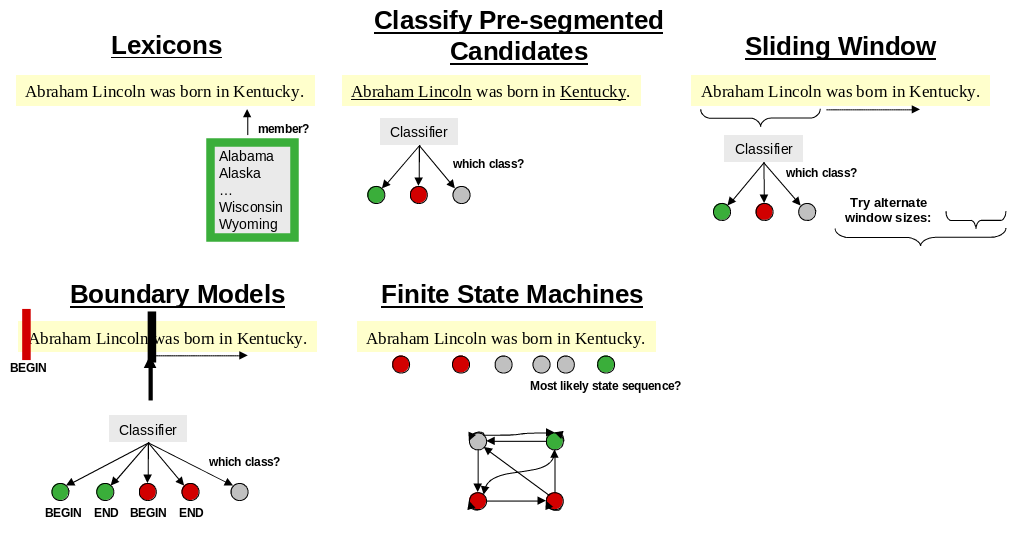
\includegraphics[height = 6cm]{cohen}\footnote{from \ref{thesurvey}}
 \end{center}

\end{frame}

 \begin{frame}
 \frametitle{NER as a sequence labeling problem}
 \begin{itemize}
  \item Observation sequence : Text \medskip
  \item State sequence : Labeling of the sequence with elements in (PER, LOC, ORG) etc. \medskip
  \item Find $\text{argmax}_{S}  P(S|O)$ \medskip
  \item Candidates : HMM, MEMM, CRF
  \end{itemize}
\end{frame}

\begin{frame}
 \frametitle{NER as a sequence labeling problem}
 \begin{itemize}
 \item \textbf{HMM} 
 \begin{itemize}
 \item Generative
 \item Makes strong independence assumption
 \item Myopic (Refer to label bias problem in \hyperref[thesurvey]{William Cohen's Survey})
 \end{itemize}
 
 \item \textbf{MEMM}
 \begin{itemize}
 \item Discriminative
 \item No independence assumptions are made, by formulation
 \item Allows the use of feature functions
 \item Myopic
 \end{itemize}
 
 \item \textbf{CRF}
 \begin{itemize}
  \item Discriminative
  \item MEMM + non myopic, avoids local normalization
  \item Talks of ``compatibility'', not independence (\hyperref[thesite]{CS 728})
 \end{itemize}

 
 \end{itemize}
 
\end{frame}